\chapter{Evaluation}
% (max 4 pages)
\section{Evaluation of the project}
% How have you evaluated/measured the success of the project? Are the requirements/expectations met? Examples: running test cases to check functionality or to evaluate performance aspects, letting other student colleagues use the project product/result and getting feedback from their user experience, comparing with alternative approaches, etc. For each requirement, you should provide a convincing argument that the project fulfils it.
% 
% Testing and playing the game
% Stress testing the connection and rendering using framerates as measure
% Timing the game components, measuring the percentage of time used on different aspects of the protocol / tick
% Letting family members and peers play the game for feedback
% 
% When an implementation is insufficient, a different approach is used. e.g. the iterative procedure of implementing collision detection, or how often the clients updated their chat.
% 
% 
% Explain how the game behaves in regards to the requirements. How does clients with slow connections effect the other players? How fast is the game approximately running? What security measures are implemented and how do they effect the program? Is the program vulnerable to attacks? Which? Is this a consequence of the program design or the tools?
% 
This section will go over each of the requirements specified in table \ref{tab:Team10Game}. Each promised feature and property and whether they're delivered by the final product will be addressed. 

\textbf{Lobby UI}\\
A screenshot of the finished \textbf{Lobby UI} can be seen in figure \ref{fig:lobbyUI} in the appendix.
The lobby UI shows players currently in the lobby (\texttt{test\_user01} and \texttt{test\_user02}) along with active rooms (\texttt{room1}). The client can pick a room from the list and click "join room" to connect to it. Alternatively clicking "create room" prompts the client to enter a name and then creates a new room with that name. \textbf{Thus the UI delivers all promised features}. The layout of the UI is very simple and it only takes 2 clicks to join a room and 3 clicks to create one. It's both easy and fast to navigate. Clicking "update" refreshes the list of online players and rooms to the newest version. \textbf{Thus the UI delivers all promised properties.}

\begin{figure}[htbp]
    \centering
    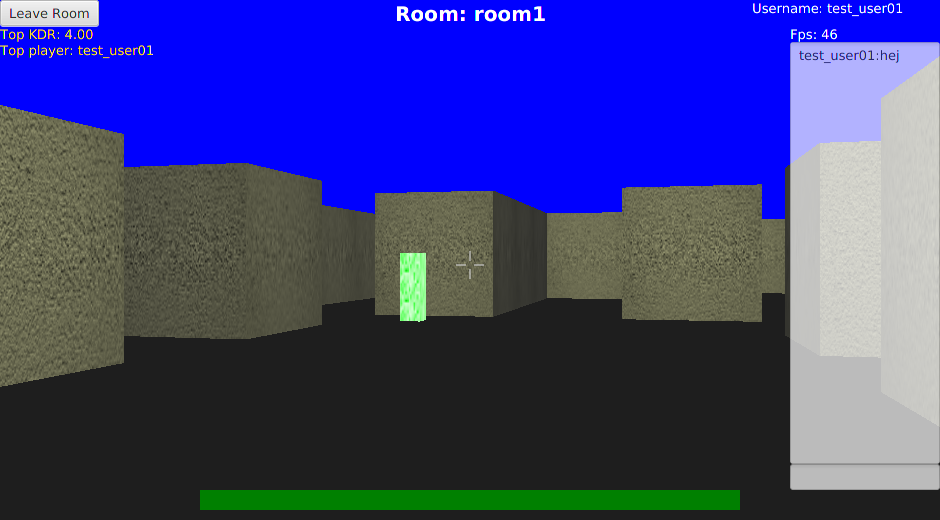
\includegraphics[width=\textwidth]{figures/room.png}
    \caption{In-game screenshot.}  
    \label{fig:game}
\end{figure}

\textbf{Core Game}\\
The finished \textbf{core game} can be seen in figure \ref{fig:game}.
When inside a room, a client can play the \textbf{core game}. She can move in real-time 360-degrees and participate with other connected clients in a free-for-all deathmatch. She can move with WASD, look around with left and right, and shoot by pressing spacebar. Shooting enemies to decrease their health and if dropped below 0 they die and respawn on a random location on the map.
Each of the promised \textbf{in-game overlay UI} elements can be seen as an overlay to the game and their values are updated regularly. \textbf{Thus the core game delivers all promised features}. We've tested the game on many different machines and everyone performed over 30FPS at all times. The latency over LAN connection is so low that collisions and movement has no noticeable delay. \textbf{Intuitive simulated physics} are provided by the robust collision system we've built. Wall-collisions feel real by only partially limiting movement parallel to the wall. The bullet collision mechanism is ultra-realistic since it uses shot-radius to collide exactly as the rendered laser-beam appears to collide to the client. \textbf{Custom maps} is not technically a feature yet, but the template-based system we've created allows for \textbf{modding} the game to play custom maps. The simplified Quake 3 Networking Model is successfully implemented meaning the client/server application is \textbf{server-authoritative}. \textbf{Thus the core game delivers all promised properties.}

\textbf{Server-side UI}\\
The finished \textbf{server-side UI} can be seen in figure \ref{fig:servermonitor} in the appendix. The \textbf{server-side UI} lists the username of all connected clients and what room they're currently in. Furthermore it lists all active rooms hosted by the server. It updates both these lists every tick and \textbf{thus the UI delivers the promised feature}. By being able to monitor all current games and see the number of clients connected to each, the user hosting the server can use this UI to see if a room thread is being overloaded or if there's too many rooms running. \textbf{Thus the UI delivers the promised property}. 



\section{Evaluation of pSpaces}
% Include a brief evaluation of pSpaces based your project experience. Have you identified limitations or bugs? Have they affected progress in your project? Have you identified/implemented potential improvements? 

The goal of this course, is to create a distributed application using \texttt{pSpaces} (in this case jSpace). During the development of the project we have gained the following experiences with this tool:

\subsection{Pros}
\texttt{pSpaces} provide an easy and approachable platform for data storage and information sharing. 

The SpaceRepository and RemoteSpaces from the framework provide a fluent transaction between local spaces and spaces accessed accross the network.

The api's are intuitive and simple to use, yet flexible enought to adopt to any communication scheme.

\subsection{Cons}
It is not possible to shield/block clients from a space added to a gate in the repository.

A malicious/clumsy client can easily empty a space, once it is added to a gate, by executing \texttt{space.getAll(...)} with templates consisting of \texttt{Object.class} as type and iteratively 1,2,3... arguments.

Since our project took inspiration from the quake networking scheme which is based on the UDP protocol, it was unfortunate that this was not yet implemented in the framework.

\subsection{Potential bugs}
\textbf{SequentialSpace class} \\
In the version of the \texttt{org.jSpace} given, the two methods \texttt{findAllTuples} and \texttt{findTuple} were not synchronized (in the java monitor) throwing occational \texttt{ConcurrentModificationException}'s when performaing e.g. \texttt{queryAll} on a \texttt{SequentialSpace}. Adding \texttt{synchronized} to the method signatures removes all the concurrent exceptions in our case. Alternatively a copy of the array/elements could be returned to seperate the framework from the usage.

\textbf{Tuple class} \\
In the \texttt{Tuple} class, occational \texttt{NullPointerException}'s were thrown. The stacktrace shows that the error occurs when \texttt{tuple.hasNext()} is called. Further investigation shows that it is the command \texttt{fields.length} which cause the error, because \texttt{fields} is \texttt{null}. To make the framework more robust, \texttt{null} checks could be introduced, to either ignore tuples with fields which are \texttt{null}, or throw an exception on creation to indicate an illegal action. To avoid this \texttt{NullPointerException} being thrown, a private parameter \texttt{length} is added to the \texttt{Tuple} class, and initialized in constructor as:
\begin{center}
\texttt{this.length = fields == null ? 0 : fields.length;}
\end{center}
and the methods are set to use this parameter instead of \texttt{fields.length}. 

\textbf{RemoteSpace}\\
When the client application exits or terminates while being connected to a \texttt{SpaceRepository}'s gate from the server application, the server would crash and throw consecutive \texttt{ConnectionResetException}'s. This may be avoided by excluding the \texttt{"?keep"} parameter in the connection, but since this project is reliant on sending information several times a second, it would be a big bottleneck to open and close the connection successively.

Lastly, when calling \texttt{queryp} on an instance of a \texttt{RemoteSpace} in the client application, the returned tuple would ocassionally neither be \texttt{null} or follow the requested template. In our case the template was composed of an actual field, and a formal field. The returned \texttt{Object[]} is checked for \texttt{null}, and afterwards the second element (index 1) of the array is accessed. This results in an \texttt{ArrayIndexOutOfBoundsException} being thrown. This can only occur if an array of length 0 or 1 is returned, which is unexpected given that the specified template has two arguments.
